% !TEX TS-program = lualatex
\documentclass[aspectratio=1610]{beamer}
\usetheme{Warsaw}
\useinnertheme{rectangles}
\useoutertheme{infolines}
\setbeamersize{text margin left=6mm,text margin right=6mm} 

\usepackage{xcolor}
\definecolor{IBMblue}{HTML}{648fff}
\definecolor{IBMviolet}{HTML}{785ef0}
\definecolor{IBMpink}{HTML}{dc267f}
\definecolor{IBMorange}{HTML}{fe6100}
\definecolor{IBMyellow}{HTML}{ffb000}
\definecolor{BleuClair}{HTML}{0078c0}
\definecolor{BleuFonce}{HTML}{222842}

\definecolor{codebg}{RGB}{240,240,240}
\definecolor{codecomment}{RGB}{0,128,0}
\definecolor{codekeyword}{RGB}{0,0,255}
\definecolor{codestring}{RGB}{255,100,0}

\setbeamercolor{palette primary}{bg=BleuFonce,fg=white}
\setbeamercolor{palette secondary}{bg=BleuFonce,fg=white}
\setbeamercolor{palette tertiary}{bg=BleuFonce,fg=white}
\setbeamercolor{palette quaternary}{bg=BleuFonce,fg=white}
\setbeamercolor{structure}{fg=BleuFonce} % itemize, enumerate, etc
\setbeamercolor{section in toc}{fg=BleuFonce} % TOC sections
% Override palette coloring with secondary
\setbeamercolor{subsection in head/foot}{bg=BleuClair,fg=white}

\usepackage[absolute,overlay]{textpos}
\usepackage{graphicx}
\usepackage[center]{caption}
\usepackage{amsfonts}
\setbeamertemplate{caption}[numbered]
\usepackage{amsmath,mathrsfs,amssymb,stmaryrd}
\usepackage{geometry}
\usepackage{pgfplots} 
\usepackage{tikz, xifthen}
\usepackage{algorithm}
\usepackage{algpseudocode}
\usepackage{animate}
\usepackage{multicol}

\usepackage{hyperref}
\usepackage[style=authoryear, backend=biber]{biblatex}
\addbibresource{biblio.bib}
\usepackage{csquotes}

\usepackage{cancel}
\usepackage{soul}
\usetikzlibrary{matrix, positioning, arrows.meta, fit}
\usepackage{fp}
\usepackage{pgfplots}
\pgfplotsset{compat=1.17}
\usepgfplotslibrary{patchplots, external}
\tikzexternalize[prefix=tikzexternal/]
\usepackage{listings}  % Ajout du package listings
\usepackage{lipsum}    % Pour le texte de remplissage (lipsum)
\usepackage[english]{babel}
\newcommand{\up}[1]{\textsuperscript{#1}}

\usepackage{empheq}


\usepackage[warnings-off={mathtools-colon,mathtools-overbracket}]{unicode-math}
\setmainfont{Fira Sans}
\setsansfont{Fira Sans}
\setmathfont{Fira Math}

\ExplSyntaxOn
\bool_gset_true:N\g__um_upGreek_bool
\bool_gset_false:N\g__um_upgreek_bool
\bool_gset_true:N\g__um_bfupGreek_bool 
\bool_gset_false:N\g__um_bfupgreek_bool 
\bool_gset_false:N \g__um_bfliteral_bool
\bool_gset_true:N  \g__um_bfupLatin_bool
\bool_gset_true:N  \g__um_upLatin_bool
\bool_gset_false:N  \g__um_bfuplatin_bool
\bool_gset_false:N  \g__um_uplatin_bool
%more if needed ...
\ExplSyntaxOff

\newcommand{\bm}[1]{\symbfit{#1}}
\newcommand{\di}{\ensuremath{\, \mathrm{d}}}
\newcommand{\e}{\ensuremath{\mathrm{e}}}


% Configuration du package listings pour le langage C
\lstdefinestyle{mystyle}{
    belowcaptionskip=1\baselineskip,
    breaklines=true,
    frame=L,
    xleftmargin=3em, % Reduced left margin
    language=C,
    showstringspaces=false,
    basicstyle=\scriptsize\ttfamily, % Smaller font size
    keywordstyle=\color{codekeyword},
    commentstyle=\color{codecomment},
    stringstyle=\color{codestring},
    backgroundcolor=\color{codebg},
    numbers=left,
    numberstyle=\tiny\color{gray},
    stepnumber=1,
    numbersep=10pt, % Reduced number separation
    captionpos=b,
    tabsize=2,
    breakatwhitespace=false,
}

\lstdefinestyle{customc}{
    belowcaptionskip=1\baselineskip,
    breaklines=true,
    frame=L,
    xleftmargin=\parindent,
    language=C,
    showstringspaces=false,
    basicstyle=\footnotesize\ttfamily,
    keywordstyle=\bfseries\color{codekeyword},
    commentstyle=\itshape\color{codecomment},
    stringstyle=\color{codestring},
    backgroundcolor=\color{codebg},
    numbers=left,
    numberstyle=\tiny\color{gray},
    stepnumber=1,
    numbersep=10pt,
    captionpos=b,
    tabsize=2,
    breakatwhitespace=false,
}


\setbeamertemplate{footline}{%
	\leavevmode\hbox{%
\begin{beamercolorbox}[wd=\paperwidth, ht=4ex,dp=2ex,leftskip=.3cm]%
{author in head/foot}%
    \usebeamerfont{author in head/foot}{\normalsize\insertframenumber/\pageref{LastPage}}
    \hfill \hspace{-4cm} \hspace{2.6cm}\usebeamerfont{author in head/foot}\insertshorttitle \hfill ~
\end{beamercolorbox}%
}
  \vskip0pt}
 
 
\logo{\hspace*{-1cm}
\includegraphics[height=0.5cm]{img/logo-embxinp.png}}

% \colorlet{bleu_item}{blue!80!green}
% \setbeamertemplate{itemize item}[square]
% \setbeamercolor{itemize item}{fg=bleu_item}
% \setbeamertemplate{frametitle continuation}{}


\hypersetup{%
	pdfauthor={Antoine BOUCHER},%
	pdftitle={Resolution of the linear Boltzmann equation by Monte Carlo method},%
	pdfsubject={MC schemes},%
	pdfcreator={Antoine BOUCHER},%
	pdfproducer={LaTeX},%
	breaklinks=true,
	pdfkeywords={Boltzmann, MC scheme},%
}%
\setbeamercolor{framesource}{fg=gray}
\setbeamerfont{framesource}{size=\tiny}
\newcommand{\source}[1]
{
	\begin{beamercolorbox}[ht=0cm,right]{framesource}
		\usebeamerfont{framesource}\usebeamercolor[fg]{framesource} Source: {#1}
	\end{beamercolorbox}
	\vspace{-6mm}	
}
\pdfstringdefDisableCommands{%
  \def\\{}%
  \def\texttt#1{<#1>}%
}

% Title Page
\setbeamerfont{title}{series=\bfseries,parent=structure}
\title{Resolution of the linear Boltzmann equation\\ by Monte Carlo method}
\subtitle{}

\author{
	Antoine Boucher\\
	Gabriel Rodiere\\
	Clément Aumonier\\
	Guillaume Doyen\\
	Khaoula El Maddah\\
	\vspace{1em}
	\textbf{Supervisor:} Gael Poette
} 
\institute{}
\date{Wednesday, 31\up{st} January 2024}
\titlegraphic{
\includegraphics[height=1cm]{img/logo-embxinp.png}}

\setbeamerfont{frametitle}{series=\bfseries,size=\large,parent=structure}

% Begin Document
\begin{document}

% Title Page
\begin{frame}[plain]
  \titlepage
\end{frame}

% Outline Slide
\begin{frame}{Table of contents}
  \tableofcontents
\end{frame}

\section{Introduction}
\begin{frame}{Fields of Application for the Boltzmann Equation}

\begin{multicols}{2}
    \begin{figure}
      \centering
      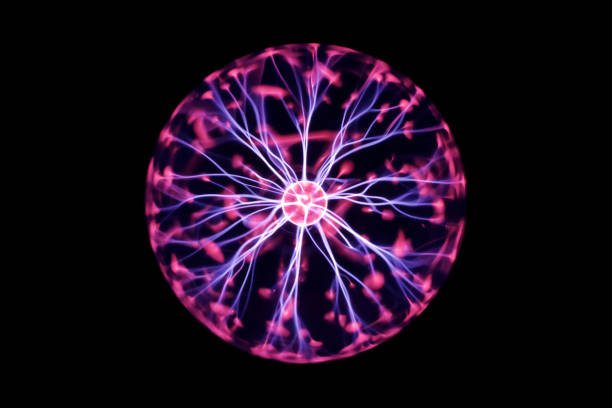
\includegraphics[width=0.6\linewidth]{img/plasma physics.jpg}
      \caption *{Plasma physics}
      
      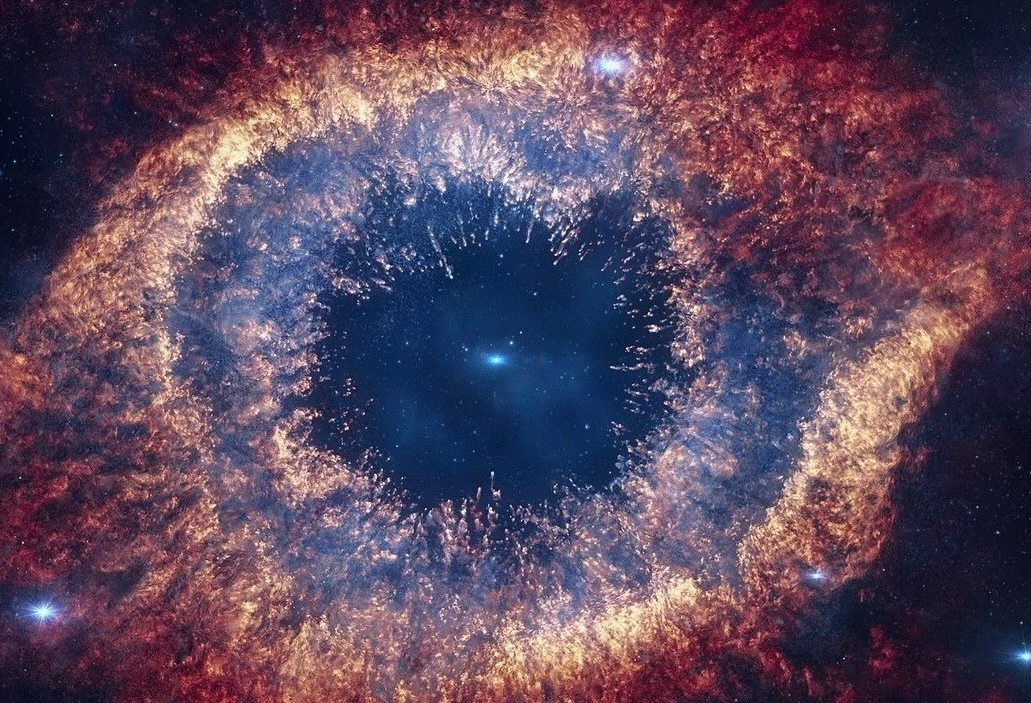
\includegraphics[width=0.6\linewidth]{img/Astrophysics.jpg}
      \caption*{Astrophysics}
    \end{figure}

    \begin{figure}
      \centering
      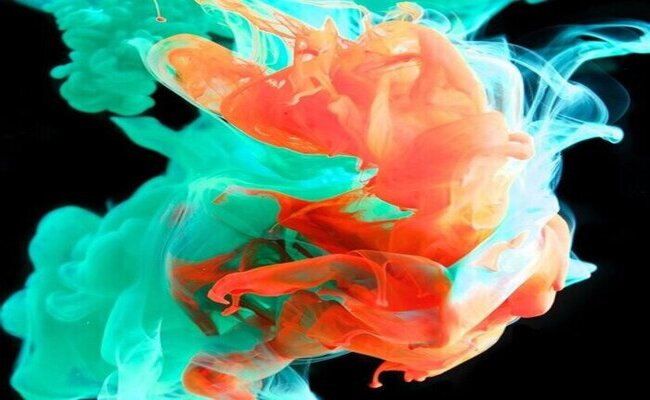
\includegraphics[width=0.6\linewidth]{img/dynamique_fluides-2.jpg}
      \caption *{Fluid dynamic}
      
      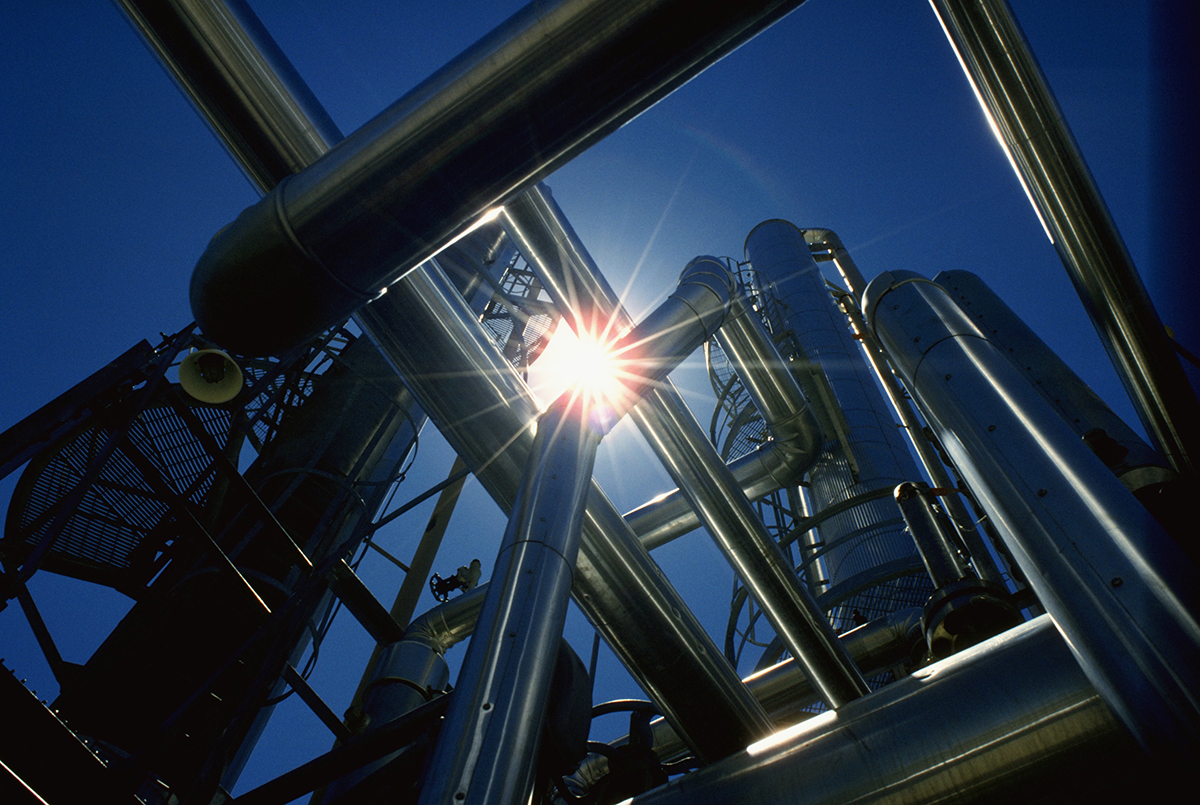
\includegraphics[width=0.6\linewidth]{img/gas.jpg}
      \caption*{Rarefied Gas Dynamics}
    \end{figure}
\end{multicols}

\end{frame}

\section{Monte Carlo method}
\begin{frame}{What is Monte Carlo?}
  \begin{figure}
    \begin{minipage}{0.48\textwidth}
      \centering
      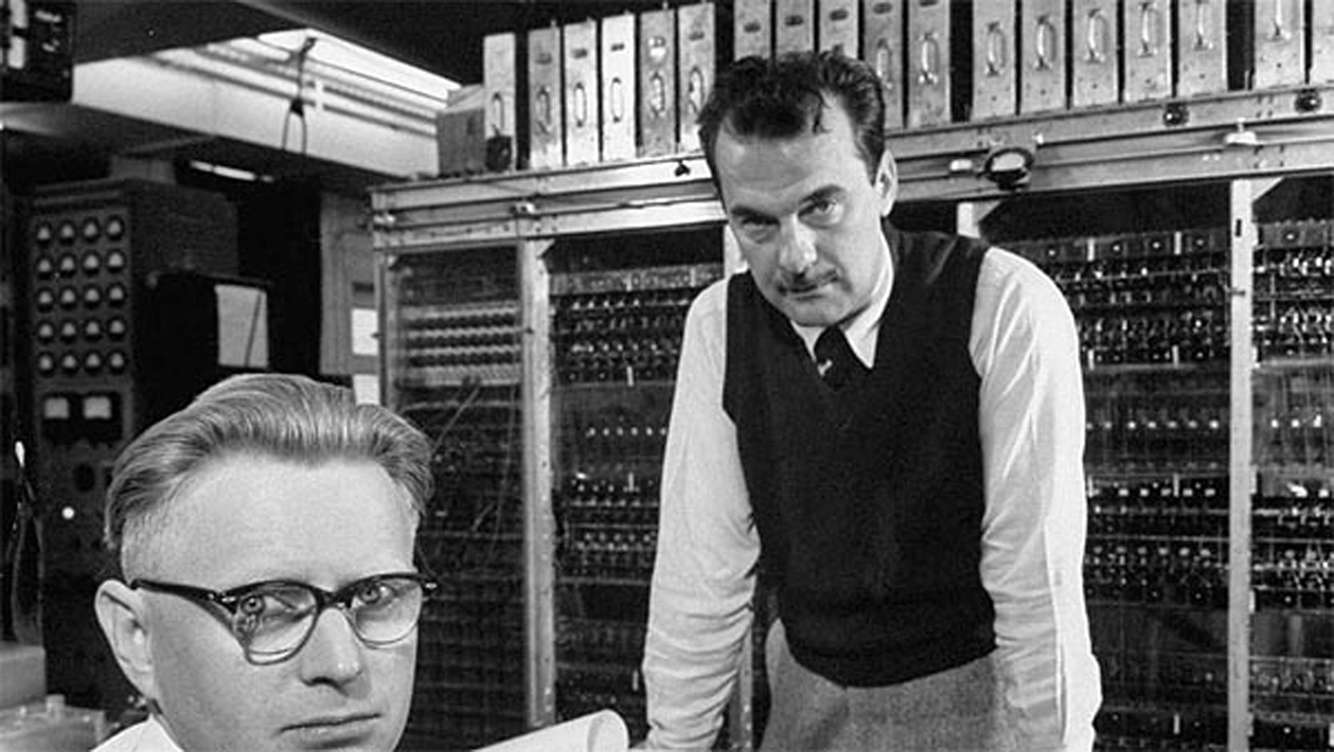
\includegraphics[width=\textwidth]{img/ch.jpg}
      \caption*{Stanislaw Ulam and Nicholas Metropolis}
      \label{fig:persons}
    \end{minipage}\hfill
    \begin{minipage}{0.48\textwidth}
      \centering
      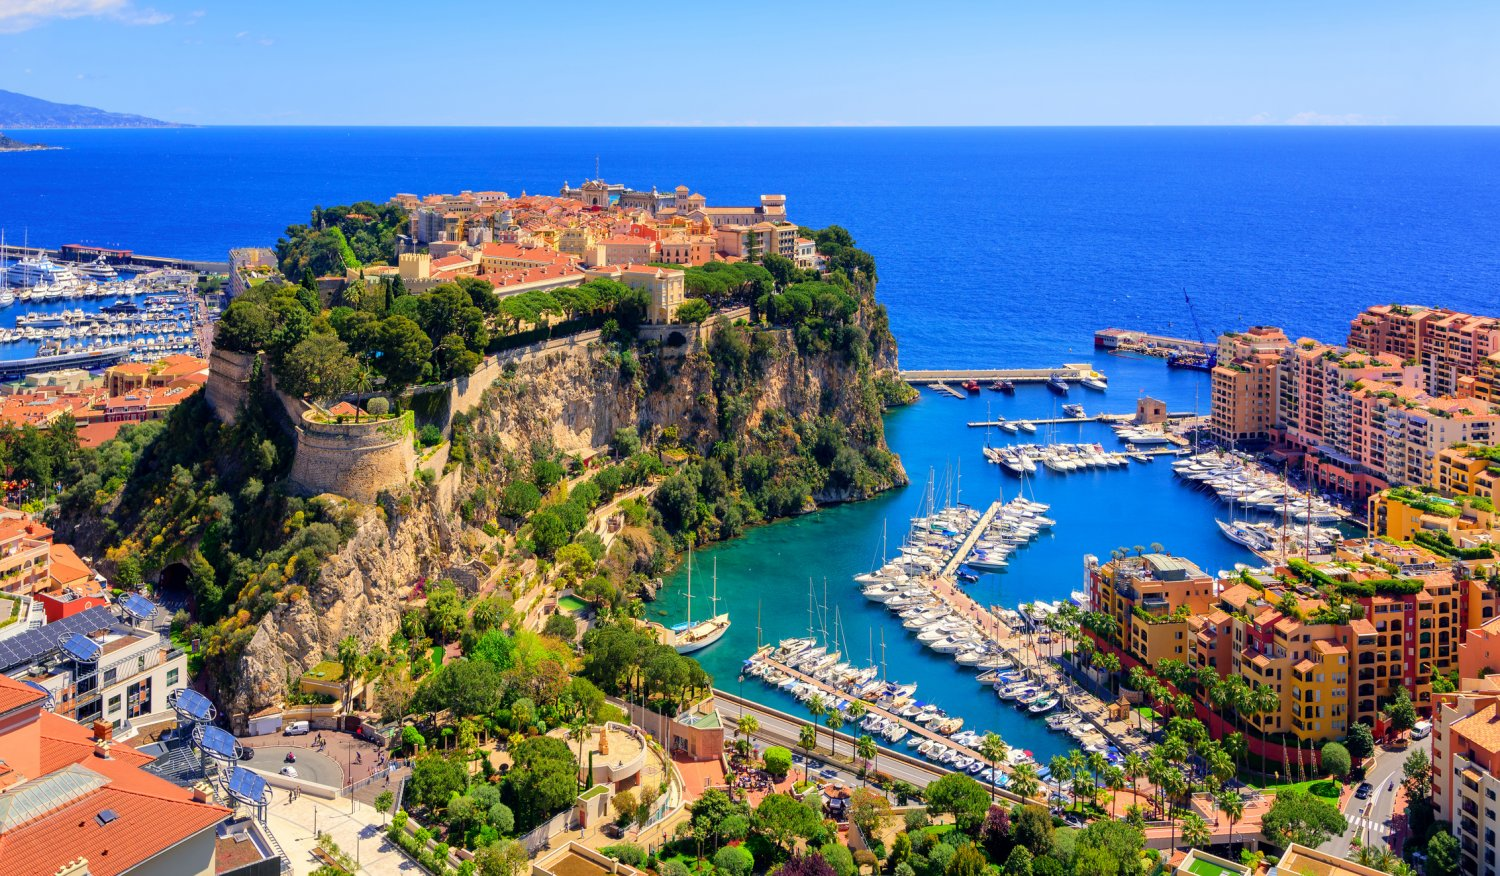
\includegraphics[width=\textwidth]{img/monte.jpg}
      \caption*{Monaco}
      \label{fig:monte}
    \end{minipage}
  \end{figure}
\end{frame}


\begin{frame}{Example of the calculation of $\pi$}
    \begin{minipage}[c]{.48\linewidth}
        \begin{figure}[h]
		  \centering
		  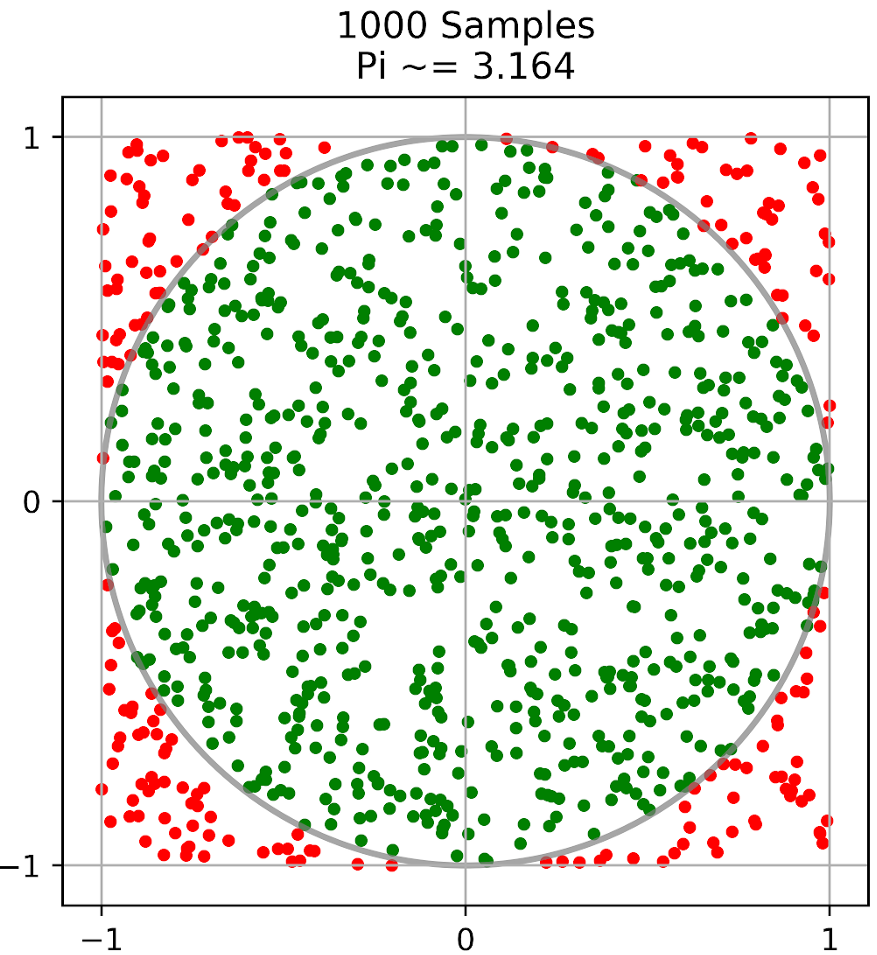
\includegraphics[width=0.85\textwidth]{img/pi.png}
		  \label{fig:circle_mc}
		\end{figure}
    \end{minipage}
    \hfill
    \begin{minipage}[c]{.48\linewidth}
         An estimate of $\pi$ is given by: 
\begin{equation*}
    \pi_N =\frac{\text{Number of stones within the circle}}{4 N}
\end{equation*}
    \end{minipage}
\end{frame}


\section{The existence and uniqueness of the solution}

\begin{frame}{Cauchy problem}
	Cauchy problem with damping $a$ and a source term $S$:
	\begin{equation*}
	\begin{cases}
	\partial_t u(\bm{x}, t, \bm{v})+\bm{v} \cdot \nabla_{\bm{x}} u(\bm{x}, t, \bm{v}) + a(\bm{x}, t, \bm{v})u(\bm{x}, t, \bm{v}) = S(\bm{x}, t, \bm{v}), \quad \bm{x} \in \mathbb{R}^n, \quad t>0.\\
	u(0,\bm{x}, \bm{v}) = u_{0}(\bm{x}, \bm{v})
	\end{cases}
	\end{equation*}
	
	\vspace{0.5cm}
	Then using the method of characteristics, we get the unique solution:\\
	
	\begin{equation*}
	u(\bm{x}, t, \bm{v}) = \left( u_0(\bm{x}-t\bm{v}, \bm{v})  + \int_0^t S(\bm{x}+(s-t)\bm{v},s,\bm{v}) \di s \right) \e^{-\int_0 ^t a(\bm{x}+(t-\tau)\bm{v}, \tau, \bm{v}) \di \tau}
	\end{equation*}
\end{frame}



\section{Resolution of the equation}
\begin{frame}{Boltzmann equation}
    The transport equation can be expressed as:
	\begin{equation*}
		\partial_t u(\bm{x},t,\bm{v}) + \bm{v} \cdot \nabla u(\bm{x},t,\bm{v}) + v\sigma_t (\bm{x},t,\bm{v})u(\bm{x},t,\bm{v})= v\sigma_s(\bm{x},t,\bm{v}) \! \int P(\bm{x},t,\bm{v},\bm{v}')u(\bm{x},t,\bm{v}') \di\bm{v}' \label{ref11}
	\end{equation*}
	\vspace{0.5cm}
	Where 
	\begin{equation*}
		\sigma_s (\bm{x},t,\bm{v})= \int \sigma_s (\bm{x},t,\bm{v},\bm{v}') \di \bm{v}', \quad  P (\bm{x},t,\bm{v},\bm{v}')= \frac{\sigma_s (\bm{x},t,\bm{v},\bm{v}')}{\sigma_s (\bm{x},t,\bm{v})}
	\end{equation*}
	$\sigma_t$: the total cross-section \\
	$\sigma_s$: the scattering cross-section \\
	$v \sigma_t$: a damping term \\
	\vspace{1em}
	\cite{noauthor_transport_2018}, \cite{poette:tel-02288678} \& \cite{lapeyre_methodes_1998}
\end{frame}

\begin{frame}{Method of characteristics}
     The initial step is re-expressing the transport equation with respect to a characteristic $\bm{x} + \bm{v}s$. It transforms into:
    \begin{equation*}
        \begin{split}
            \partial _s u(\bm{x}+\bm{v}s,s,\bm{v}) &= -v\sigma_t (\bm{x}+\bm{v}s,s,\bm{v})u(\bm{x}+\bm{v}s,s,\bm{v}) \\
            &\quad + v\sigma_s(\bm{x}+\bm{v}s,s,\bm{v})\int P (\bm{x}+\bm{v}s,s,\bm{v},\bm{v}')u(\bm{x}+\bm{v}s,s,\bm{v}')\di\bm{v}'
        \end{split}
    \end{equation*}
    
    After multiplying both sides of the equation by:
    \begin{equation*}
    	\e^{\int _0^s v\sigma_t (\bm{x} + \bm{v}\alpha,\alpha, v) \di \alpha}
    \end{equation*}
    

    Following that, we obtain:
    \begin{equation*}
    	\begin{split}
    		&\partial _s [u(\bm{x}+\bm{v}s,s,\bm{v})\e^{\int _0^s v\sigma_t (\bm{x} + \bm{v}\alpha,\alpha, v) \di \alpha}] \\
    		&= \e^{\int _0^s v\sigma_t (\bm{x} + \bm{v}\alpha,\alpha, v) \di\alpha} v\sigma_s(\bm{x}+\bm{v}s,s,\bm{v})\int P (\bm{x}+\bm{v}s,s,\bm{v},\bm{v}')u(\bm{x}+\bm{v}s,s,\bm{v}') \di \bm{v}'
    	\end{split}
    \end{equation*}
\end{frame}

\begin{frame}{Integration of the equation}
    We get after integrating the equation between $(0, t)$:
    \vspace{-1em}
    \begin{multline*}
        u(\bm{x}+\bm{v}t,t,\bm{v}) = u_0(\bm{x}, \bm{v}) \exp\left(- \int_{0}^{t} v\sigma_t\left(\bm{x} + \bm{v} \alpha, \alpha, \bm{v}\right) \di\alpha\right) \\
        + \int_{0}^{t} \int v\sigma_s\left(\bm{x} + \bm{v}s, s, \bm{v}\right) u\left(\bm{x} + \bm{v}s, s, \bm{v}'\right) \e^{- \int_s^t v\sigma_t\left(\bm{x} + \bm{v} \alpha, \bm{v}\right) \di\alpha} P\left(\bm{x} + \bm{v} s, s, \bm{v}, \bm{v}'\right) \di\bm{v}' \di s
    \end{multline*}
	
     After a variable change, we obtain:
     \vspace{-1em}
    \begin{multline*}
        u(\bm{x},t,\bm{v}) = u_0(\bm{x} - \bm{v}t, \bm{v}) \exp\left(- \int_{0}^{t} v\sigma_t\left(\bm{x} - \bm{v}(t - \alpha), \alpha, \bm{v}\right) \do\alpha\right) \\
        + \int_{0}^{t} \int v\sigma_s\left(\bm{x} - \bm{v}(t - s), s, \bm{v}\right) u\left(\bm{x} - \bm{v}(t - s), s, \bm{v}'\right) \\
        \e^{- \int_s^t v\sigma_t\left(x - \bm{v}(t - \alpha), \bm{v}\right) \di\alpha} P\left(\bm{x} - \bm{v}(t - s), s, \bm{v}, \bm{v}'\right) \di\bm{v}' \di s
    \end{multline*}
\end{frame}

%\begin{frame}{Re-expression of the exponential}
%    We also have:
%    \vspace{0.5cm}
%    \begin{multline*}
%        \exp\left(- \int_{0}^{t} v\sigma_t\left(x - \bm{v}(t - \alpha), \alpha, \bm{v}\right) \di \alpha\right) = \exp\left(- \int_{0}^{t} v\sigma_t\left(x - \bm{v} \alpha,t- \alpha, \bm{v}\right) \di \alpha\right) \\ 
%        = \int _t^\infty  v\sigma_t\left(x - \bm{v} s,t- s, \bm{v}\right)
%        \exp\left(- \int_{0}^{s} v\sigma_t\left(x - \bm{v} \alpha,t- \alpha, \bm{v}\right) \di\alpha\right) \di s
%    \end{multline*}
%\end{frame}
\begin{frame}{The integral form of the Boltzmann equation}
    The integral representation of the transport equation is then provided by:
    \begin{multline*}
        u(x,t,\bm{v}) =  \int _t^\infty  u_0(\bm{x} - \bm{v}t, \bm{v}) v\sigma_t\left(\bm{x} - \bm{v} s,t- s, \bm{v}\right) \exp\left(- \int_{0}^{s} v\sigma_t\left(\bm{x} - \bm{v} \alpha,t- \alpha, \bm{v}\right) \di\alpha\right) \di s\\
        + \int_{0}^{t} \int v\sigma_s\left(\bm{x} - \bm{v}(t - s), s, \bm{v}\right) u\left(\bm{x} - \bm{v}(t - s), s, \bm{v}'\right) \\
        \e^{- \int_s^t v\sigma_t\left(\bm{x} - \bm{v}(t - \alpha), \bm{v}\right) \di\alpha} P\left(\bm{x} - \bm{v}(t - s), s, \bm{v}, \bm{v}'\right) \di \bm{v}' \di s \label{ref13}
    \end{multline*}

    \vspace{1em}
    \centering
    \fbox{\parbox{0.7\textwidth}{\centering\textbf{Problem: the solution depends on its own integral!} \\
   	\raisebox{2.5pt}{$\Rdsh$} Let's introduce a recursive numerical MC scheme!}}
\end{frame}

\section{The semi-analog MC scheme}
\begin{frame}{Semi-analog scheme}
    For the semi-analog scheme, well used in Neutronics, we introduce the probability measure of the interaction time: 
    \begin{equation*}
    f_{\tau}(\bm{x}, t, \bm{v}, s) \di s = 1_{[0,\infty[}(s) \, v\sigma_t(\bm{x} - \bm{v}s, t - s, v) \e^{-\int_{0}^s v\sigma_t(\bm{x} - \bm{v}\alpha, t - \alpha, v) \, \di \alpha} \di s
    \end{equation*}
    for all $(\bm{x}, t, \bm{v}) \in D \times (0, T) \times \mathbb{R}^3$\\
    \vspace{1.0cm}
    We introduce the specified random variables:
    \vspace{0.5cm}
    \begin{equation*}
        \left\{
            \begin{array}{ll}
                \tau \text{ with probability measure } f_{\tau}(\bm{x}, t, \bm{v}) \, \di s, \\
                \bm{V}' \text{ with probability measure } P_{\bm{V}'}^{s}(\bm{x}, t, s, \bm{v}, \bm{v}') \, \di v'
            \end{array}
        \right.
    \end{equation*}
\end{frame}

\begin{frame}{Expression of the solution}
	We found the following \textbf{expectation} value:
	    \begin{equation*}
	            u(\bm{x}, t, \bm{v}) = \mathbb{E} \left[1_{[t, \infty[}(\tau) \: u_0(\bm{x} - \bm{v}t, \bm{v}) + 1_{[0, t[}(\tau) \: \frac{\sigma_s(\bm{x} - \bm{v}\tau, t - \tau, \bm{v})}{\sigma_t(\bm{x} - \bm{v}\tau, t - \tau, \bm{v})}u(\bm{x} - \bm{v}\tau, t - \tau, \bm{V}')\right]
	    \end{equation*}
	We seek solutions that possess this specific structure:
	\begin{equation*}
	u_p(\bm{x},t,\bm{v}) = w_p(t)\: \delta_x(\bm{x}_p(t)) \:\delta_{\bm{v}}(\bm{v}_p(t)) 
	\end{equation*}
	Replacing \(u_p\) in the equation yields:
	\begin{empheq}[left=\empheqbiglbrace]{align*}
	w_p(t) &= 1_{[0,\infty[}(\tau)w_p(0) + 1_{[0,t[}(\tau) \frac{\sigma_s}{\sigma_t} \left(
	\bm{x}_p(t-\tau),t-\tau,\bm{v}_p(t-\tau) \right) w_p(t-\tau),\\
	\bm{x}_p(t) &= 1_{[0,\infty[}(\tau)(\bm{x}_0-\bm{v}t) + 1_{[0,t[}(\tau)(\bm{x}_{t-\tau}-\bm{v}\tau),\\
	\bm{v}_p(t) &= 1_{[0,\infty[}(\tau)\bm{v} + 1_{[0,t[}(\tau)\bm{V}'. 
	\end{empheq}
\end{frame}

\begin{frame}[fragile]{Monte Carlo Particle Transport Algorithm}
	\setlength{\columnsep}{-1.5cm}
    \begin{multicols}{2}
    	\algrenewcommand\algorithmicindent{0.3em}%
        \begin{algorithmic}[1]
                \State Let $u(\bm{x}, t, \bm{v}) \gets 0$;
                \For{$p \in \llbracket 1 ; N_{MC} \rrbracket$}
                    \State set $s_p = t$
                    \State set $\bm{x}_p = \bm{x}$
                    \State set $\bm{v}_p = \bm{v}$
                    \State set $w_p(t) = N_{MC}$
                    \While{$s_p > 0$ and $w_p > 0$}
                        \If{$\bm{x}_p \not \in \mathcal{D}$}
                            \State apply\_BCs$(\bm{x}_p, s_p, \bm{v}_p)$
                        \EndIf
                        \State Sample $\tau \leadsto f_\tau(\bm{x}_p, s_p, \bm{v}_p, s) \di s$
                        \newcolumn
                        \If{$\tau < s_p$}
	                        \Comment{{\scriptsize \leftarrow Scattering/Collision}}
	                        \State $w_p \gets \frac{\sigma_s(\bm{x}_p, s_p - \tau, \bm{v}_p)}{\sigma_t(\bm{x}_p, s_p - \tau, \bm{v}_p)} w_p$
	                        \State Sample $\bm{v}_p \leadsto P_{\bm{V}'}^s(\bm{x}_p, s_p, \tau, \bm{v}_p, \bm{v}') \di \bm{v}'$
	                        \State $\bm{x}_p \gets \bm{x}_p + \bm{v}_p \tau$
	                        \State $s_p \gets s_p - \tau > 0$
                        
                        \Else
                       		\Comment{{\scriptsize \leftarrow Census/Contribution}}
                            \State $\bm{x}_p \gets \bm{x}_p + s_p \bm{v}_p$
                            \State $s_p \gets 0$
                            \State $u(\bm{x}, t, \bm{v}) += w_p u_0(\bm{x}_p, \bm{v}_p)$
                        \EndIf
                    \EndWhile
                \EndFor
        \end{algorithmic}
    \end{multicols}
\end{frame}

\section{Tests}

\begin{frame}{Architecture of the code}
	\begin{figure}
		\centering
		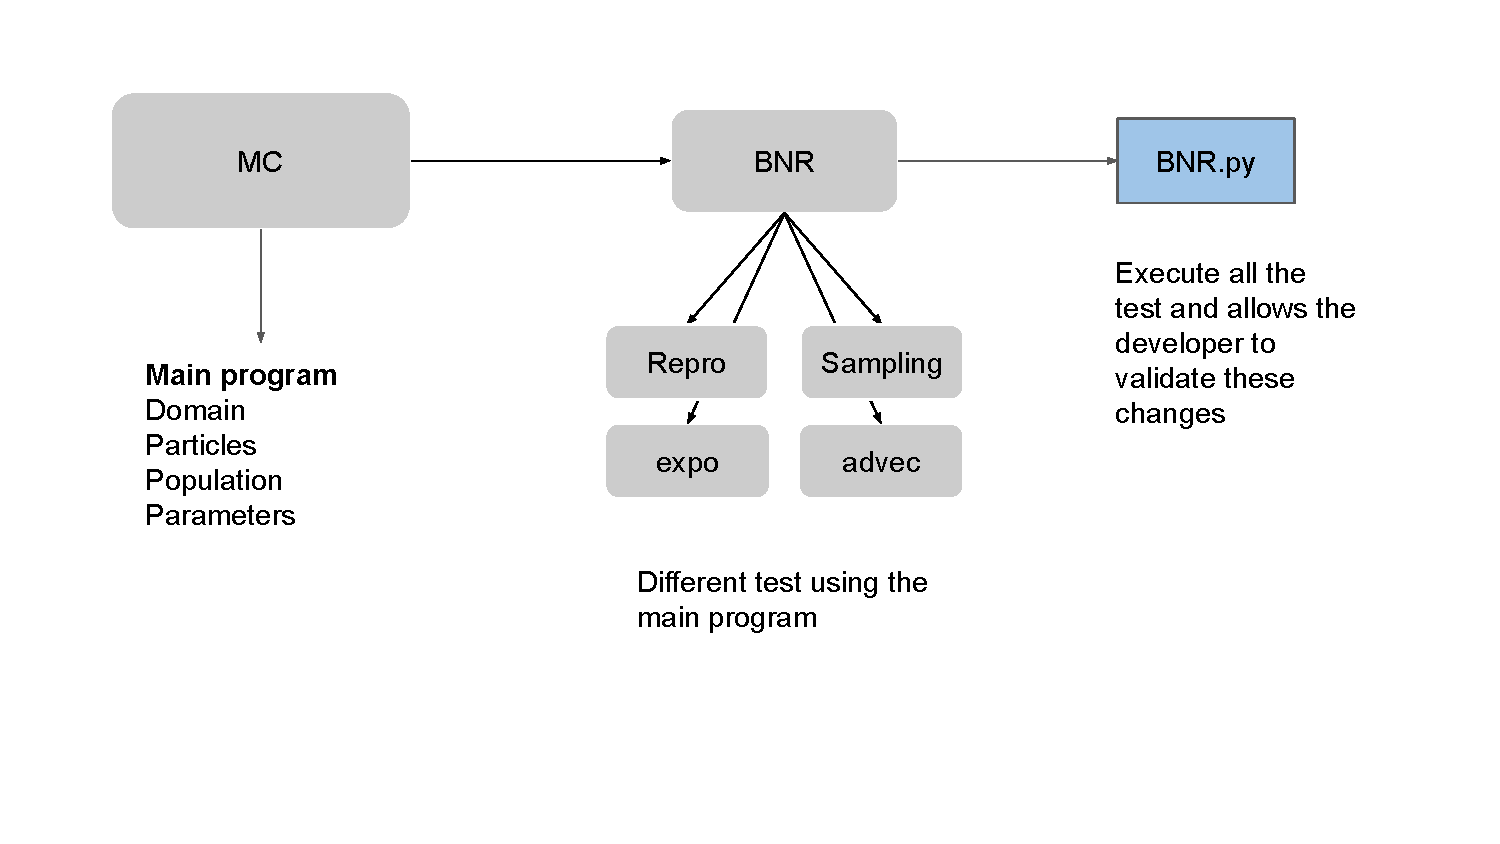
\includegraphics[height=0.7\textheight]{img/codestruct.pdf}
		\label{fig:code_structure}
	\end{figure}
\end{frame}

\begin{frame}[fragile]{Samplings of $\tau$ and $\bm{v}_p$}
	\setlength{\columnsep}{-2cm}
	\begin{multicols}{2}
		\vspace*{3em}
		The variables are sampled as follows:
		\vspace{1em}
		
		 $\tau = - \frac{\log U}{\sigma_t(\bm{x}_p, s_p, \bm{v}_p) |\bm{v}_p|}$ where $U \leadsto \mathcal{U}[0;1]$.
		 
		\vspace{1em}
		
		$\bm{v}_p$ is sampled uniformly on the 3D \\ unit sphere.
		\newcolumn
		\vspace*{-5em}
		
		\begin{figure}[H]
			% fix axes to these ranges (depending on the data to be plotted, of course)
			\def\xmin{-1.5}
			\def\xmax{1.5}
			\def\ymin{-1.5}
			\def\ymax{1.5}
			\def\zmin{-1.5}
			\def\zmax{1.5}
			% bounding cylinder based on axes ranges with some scaling and z-offsets to also
			% include tick labels
			\def\scaleCylRadius{1.5}
			\pgfmathsetmacro\cylCentreX{0.5*(\xmin+\xmax)}
			\pgfmathsetmacro\cylCentreY{0.5*(\ymin+\ymax)}
			\pgfmathsetmacro\cylRadius{\scaleCylRadius*sqrt((\xmax-\xmin)^2+(\ymax-\ymin)^2))/2}
			\pgfmathsetmacro\cylZMin{\zmin - 0.02}
			\pgfmathsetmacro\cylZMax{\zmax + 0.0}
			
			\centering
			\begin{animateinline}[autoplay,loop,controls=none]{12} 
				\multiframe{36}{i=45+10}{
					\begin{tikzpicture} 
						%\useasboundingbox (-5,-5) rectangle (5, 5);
						\begin{axis}[%
							grid = both,
							major grid style = {lightgray},
							minor grid style = {lightgray!25},
							height = 0.8\textheight,
							xlabel = {x},
							ylabel = {y},
							zlabel = {z},
							title = {},
							legend style={at={(0.5,1)},anchor=north},
							xmin=\xmin,xmax=\xmax,
							ymin=\ymin,ymax=\ymax,
							zmin=\zmin,zmax=\zmax,
							view={\i}{30},
							clip=false,
							trig format plots=rad,
							%unit vector ratio = 1 1 1
							]
							
							% lower circle
							\addplot3[
							draw=none, % comment out to see cylinder circles
							domain=0:2*pi,samples=60]({\cylCentreX+\cylRadius*sin(x)},{\cylCentreY+\cylRadius*cos(x)},\cylZMin);
							
							\addplot3 [color=IBMblue, only marks, mark size = 1pt] table [col sep=space, x index=0, y index=1, z index=2] {plot/data1500.txt};
							
							\draw[-stealth, color=IBMviolet, ultra thick] (0.0,0.0,0.0) -- (1.5, 0.0, 0.0) {};
							\draw[-stealth, color=IBMviolet, ultra thick] (0.0,0.0,0.0) -- (0.0, 1.5, 0.0) {};
							\draw[-stealth, color=IBMviolet, ultra thick] (0.0,0.0,0.0) -- (0.0, 0.0, 1.5) {};
							
							% upper circle
							\addplot3[
							draw=none,
							domain=0:2*pi,samples=60]({\cylCentreX+\cylRadius*sin(x)},{\cylCentreY+\cylRadius*cos(x)},\cylZMax);
							\legend{};
						\end{axis}
					\end{tikzpicture} 
				} 
			\end{animateinline} 
		\end{figure}
	\end{multicols}
\end{frame}

\section{Numerical results}

\begin{frame}{1D results}
\begin{figure}[h]
  \centering
  \begin{tikzpicture}
		\begin{axis}[%
			very thick,
			grid = both,
			major grid style = {lightgray},
			minor grid style = {lightgray!25},
			width = 0.9\textwidth,
			height = 0.8\textheight,
			xlabel = {x},
			ylabel = {Solution $u(x, t, v)$},
			legend style={at={(1,1)},anchor=north east},
			legend cell align={left},
            xmin = -1.0,
            xmax = 1.0,
            ymin = 0
			]
   
			\addplot[color=IBMblue, mark=none] table [col sep=space, x index=0, y index=3] {plot/solution_t_1.000000_nb_10.txt};
            \addplot[color=IBMorange, mark=none] table [col sep=space, x index=0, y index=3] {plot/solution_t_1.000000_nb_100.txt};
            \addplot[color=IBMpink, mark=none] table [col sep=space, x index=0, y index=3] {plot/solution_t_1.000000_nb_100000.txt};

        \legend{$N_{MC} = 10$,%
        $N_{MC} = 100$,
        $N_{MC} = 10000$,};
		\end{axis}
	\end{tikzpicture}
  \label{fig:visualisation1D}
  \caption{Solution refinement with $N_{MC}$ in 1D.}
\end{figure}
\end{frame}

\begin{frame}{1D results}
\begin{figure}[h]
  \centering
  \begin{tikzpicture}
		\begin{axis}[%
			very thick,
			grid = both,
			major grid style = {lightgray},
			minor grid style = {lightgray!25},
			width = 0.9\textwidth,
			height = 0.8\textheight,
			xlabel = {t},
			ylabel = {Solution $u(0, t, v)$},
			legend style={at={(0.0,0.0)},anchor=south west},
			legend cell align={left},
            %xmin = -1.0,
            %xmax = 1.0,
            ymin = 0
			]

			\addplot[color=IBMorange, mark=none, domain=0:0.9] {5.0}; 
			\addplot[color=IBMblue, mark=+, only marks, mark size=4pt] table [col sep=space, x index=0, y index=7] {plot/solution_depends_t.txt} node[color=black, below] at (0.8, 5) {$\sigma_s = 0, \sigma_t=0$};
			
			\addplot[color=IBMorange, mark=none, domain=0:0.9] {5.0*exp(-0.5*x)}; 
			\addplot[color=IBMblue, mark=+, only marks, mark size=4pt] table [col sep=space, x index=0, y index=6] {plot/solution_depends_t.txt} node[color=black, below, align=right, rotate=-7] at (0.8, 3.3) {$\sigma_s = 0.5, \sigma_t= 1$};
			
            \addplot[color=IBMorange, mark=none, domain=0:0.9] {5.0*exp(-x)}; 
			\addplot[color=IBMblue, mark=+, only marks, mark size=4pt] table [col sep=space, x index=0, y index=4] {plot/solution_depends_t.txt} node[anchor=east,color=black, below,rotate=-10] at (0.8, 2.25) {$\sigma_s = 0, \sigma_t=1$};
			
			

        \legend{$u_0 \e^{-|\bm{v}|(\sigma_t - \sigma_s) t}$, MC scheme};
		\end{axis}
	\end{tikzpicture}
  \label{fig:visualisation_temps}
  \caption{Solution in 1D over time with an intermediate regime.}
\end{figure}
\end{frame}

\begin{frame}{1D results}
\begin{figure}[h]
	\centering
	\begin{animateinline}[autoplay,loop,controls=none]{3} 
		\multiframe{11}{i=0+1}{
		\begin{tikzpicture}
			\begin{axis}[%
				very thick,
				grid = both,
				major grid style = {lightgray},
				minor grid style = {lightgray!25},
				width = 0.9\textwidth,
				height = 0.8\textheight,
				xlabel = {x},
				ylabel = {Solution $u(x, t, v)$},
				legend style={at={(1,1)},anchor=north east},
				legend cell align={left},
				xmin = 0.0,
				xmax = 2.0,
				ymin = 0
				]
				
				\addplot[color=IBMblue, mark=none] table [col sep=space, x index=0, y index=4] {plot/advection1D/solution_t_\i.txt};
				
				\legend{$N_{MC} = 10000$,};
			\end{axis}
		\end{tikzpicture}
		}
	\end{animateinline} 
	\label{fig:visualisation1D_advection}
	\caption{Solution in 1D with $\sigma_s = \sigma_t = 0$.}
\end{figure}
\end{frame}

\begin{frame}{2D Transparent medium}
	When $\sigma_t = \sigma_s = 0$, the explicit solution is given, with a \textbf{gaussian} initial solution by: 
	\begin{equation*}
		u(\bm{x},t,\bm{v}) = u_0(\bm{x}-\bm{v}t, \bm{v})
	\end{equation*}
	\vspace{-2em}
	\begin{figure}[H]
		\centering
		\begin{animateinline}[autoplay,loop,controls=none]{3} 
			\multiframe{11}{i=0+1}{
				  \begin{tikzpicture}
							\begin{axis}[%
									%very thick,
									grid = both,
									major grid style = {lightgray},
									minor grid style = {lightgray!25},
									%width = 0.7\textwidth,
									height = 0.8\textheight,
									xlabel = {x},
									ylabel = {y},
						            title = {},
									legend style={at={(0.5,1)},anchor=north},
						            xmin = -1.0,
						            xmax = 1.0,
						            ymin = -1.0,
						            ymax = 1.0,
						            zmin = 0.0,
						            zmax = 1.0,
						            view={110}{25},
						            mesh/ordering=x varies,
						            mesh/rows=60,
						            colorbar,
						            point meta min=0.0,
						            point meta max=1.0,
						            colormap/viridis,
						            %shader=interp,
						            %patch type=bilinear,
									]
						   
									\addplot3 [color=IBMblue, surf, opacity=1, fill opacity=1] table [col sep=space, x index=0, y index=1, z index=4] {plot/advection/solution_t_\i.txt};
						
						        %\legend{$\texttt{nbMC} = 10$,};
								\end{axis}
						\end{tikzpicture}
			}
		\end{animateinline} 
	\end{figure}
\end{frame}
\begin{frame}{2D Absorbing medium}
	When $\sigma_s = 0$ and $\sigma_t = 1$, an exact solution is known:
	\begin{equation*}
		u(\bm{x}, t, \bm{v}) = \left( u_0(\bm{x}-t\bm{v}, \bm{v}) \right) \e^{-\int_0 ^t v\sigma_t(\bm{x}+(t-\tau)\bm{v}, \tau, \bm{v}) \di \tau}
	\end{equation*}
	\vspace{-2em}
	\begin{figure}[H]
		\centering
		\begin{animateinline}[autoplay,loop,controls=none]{3} 
			\multiframe{11}{i=0+1}{
				\begin{tikzpicture}
					\begin{axis}[%
						%very thick,
						grid = both,
						major grid style = {lightgray},
						minor grid style = {lightgray!25},
						%width = 0.7\textwidth,
						height = 0.8\textheight,
						xlabel = {x},
						ylabel = {y},
						title = {},
						legend style={at={(0.5,1)},anchor=north},
						xmin = -1.0,
						xmax = 1.0,
						ymin = -1.0,
						ymax = 1.0,
						zmin = 0.0,
						zmax = 1.0,
						view={110}{25},
						mesh/ordering=x varies,
						mesh/rows=60,
						colorbar,
						point meta min=0.0,
						point meta max=1.0,
						colormap/viridis,
						%shader=interp,
						%patch type=bilinear,
						]
						
						\addplot3 [color=IBMblue, surf, opacity=1, fill opacity=1] table [col sep=space, x index=0, y index=1, z index=4] {plot/absorption/solution_t_\i.txt};
						
						%\legend{$\texttt{nbMC} = 10$,};
					\end{axis}
				\end{tikzpicture}
			}
		\end{animateinline} 
	\end{figure}
\end{frame}

\begin{frame}{2D Absorption-scattering medium}
	With $\sigma_s = 0.5$ and $\sigma_t = 1$: \textbf{no exact solution} is known.
	\begin{figure}[H]
		\centering
		\begin{animateinline}[autoplay,loop,controls=none]{3} 
			\multiframe{11}{i=0+1}{
				\begin{tikzpicture}
					\begin{axis}[%
						%very thick,
						grid = both,
						major grid style = {lightgray},
						minor grid style = {lightgray!25},
						%width = 0.7\textwidth,
						height = 0.8\textheight,
						xlabel = {x},
						ylabel = {y},
						title = {},
						legend style={at={(0.5,1)},anchor=north},
						xmin = -1.0,
						xmax = 1.0,
						ymin = -1.0,
						ymax = 1.0,
						zmin = 0.0,
						zmax = 1.0,
						view={110}{25},
						mesh/ordering=y varies,
						mesh/rows=60,
						colorbar,
						point meta min=0.0,
						point meta max=1.0,
						colormap/viridis,
						%shader=interp,
						%patch type=bilinear,
						]
						
						\addplot3 [color=IBMblue, surf, opacity=1, fill opacity=1] table [col sep=space, x index=0, y index=1, z index=4] {plot/scattering/solution_t_\i.txt};
						
						%\legend{$\texttt{nbMC} = 10$,};
					\end{axis}
				\end{tikzpicture}
			}
		\end{animateinline} 
	\end{figure}
\end{frame}



\section{Conclusion}
\begin{frame}{Conclusion}
	\textbf{Main interests of MC schemes:}
	\begin{itemize}
		\item uses recursive formulation,
		\item 2D/3D w/o extra cost,
		\item multiple schemes (\textbf{backward here for shields in radioprotection}/forward, analog/semi-analog/non-analog) depending on the application,
		\item immediate parallelization thanks to independent particles.
	\end{itemize}
	\vspace{1em}
	
	\textbf{Possible improvements:}
	\begin{itemize}
		\item elaborate more tests,
		\item implement the forward scheme for more boundary conditions.
	\end{itemize}
	\label{LastPage}
\end{frame}

\begin{frame}[plain]{Website}
	
	\begin{figure}[H]
		\centering
		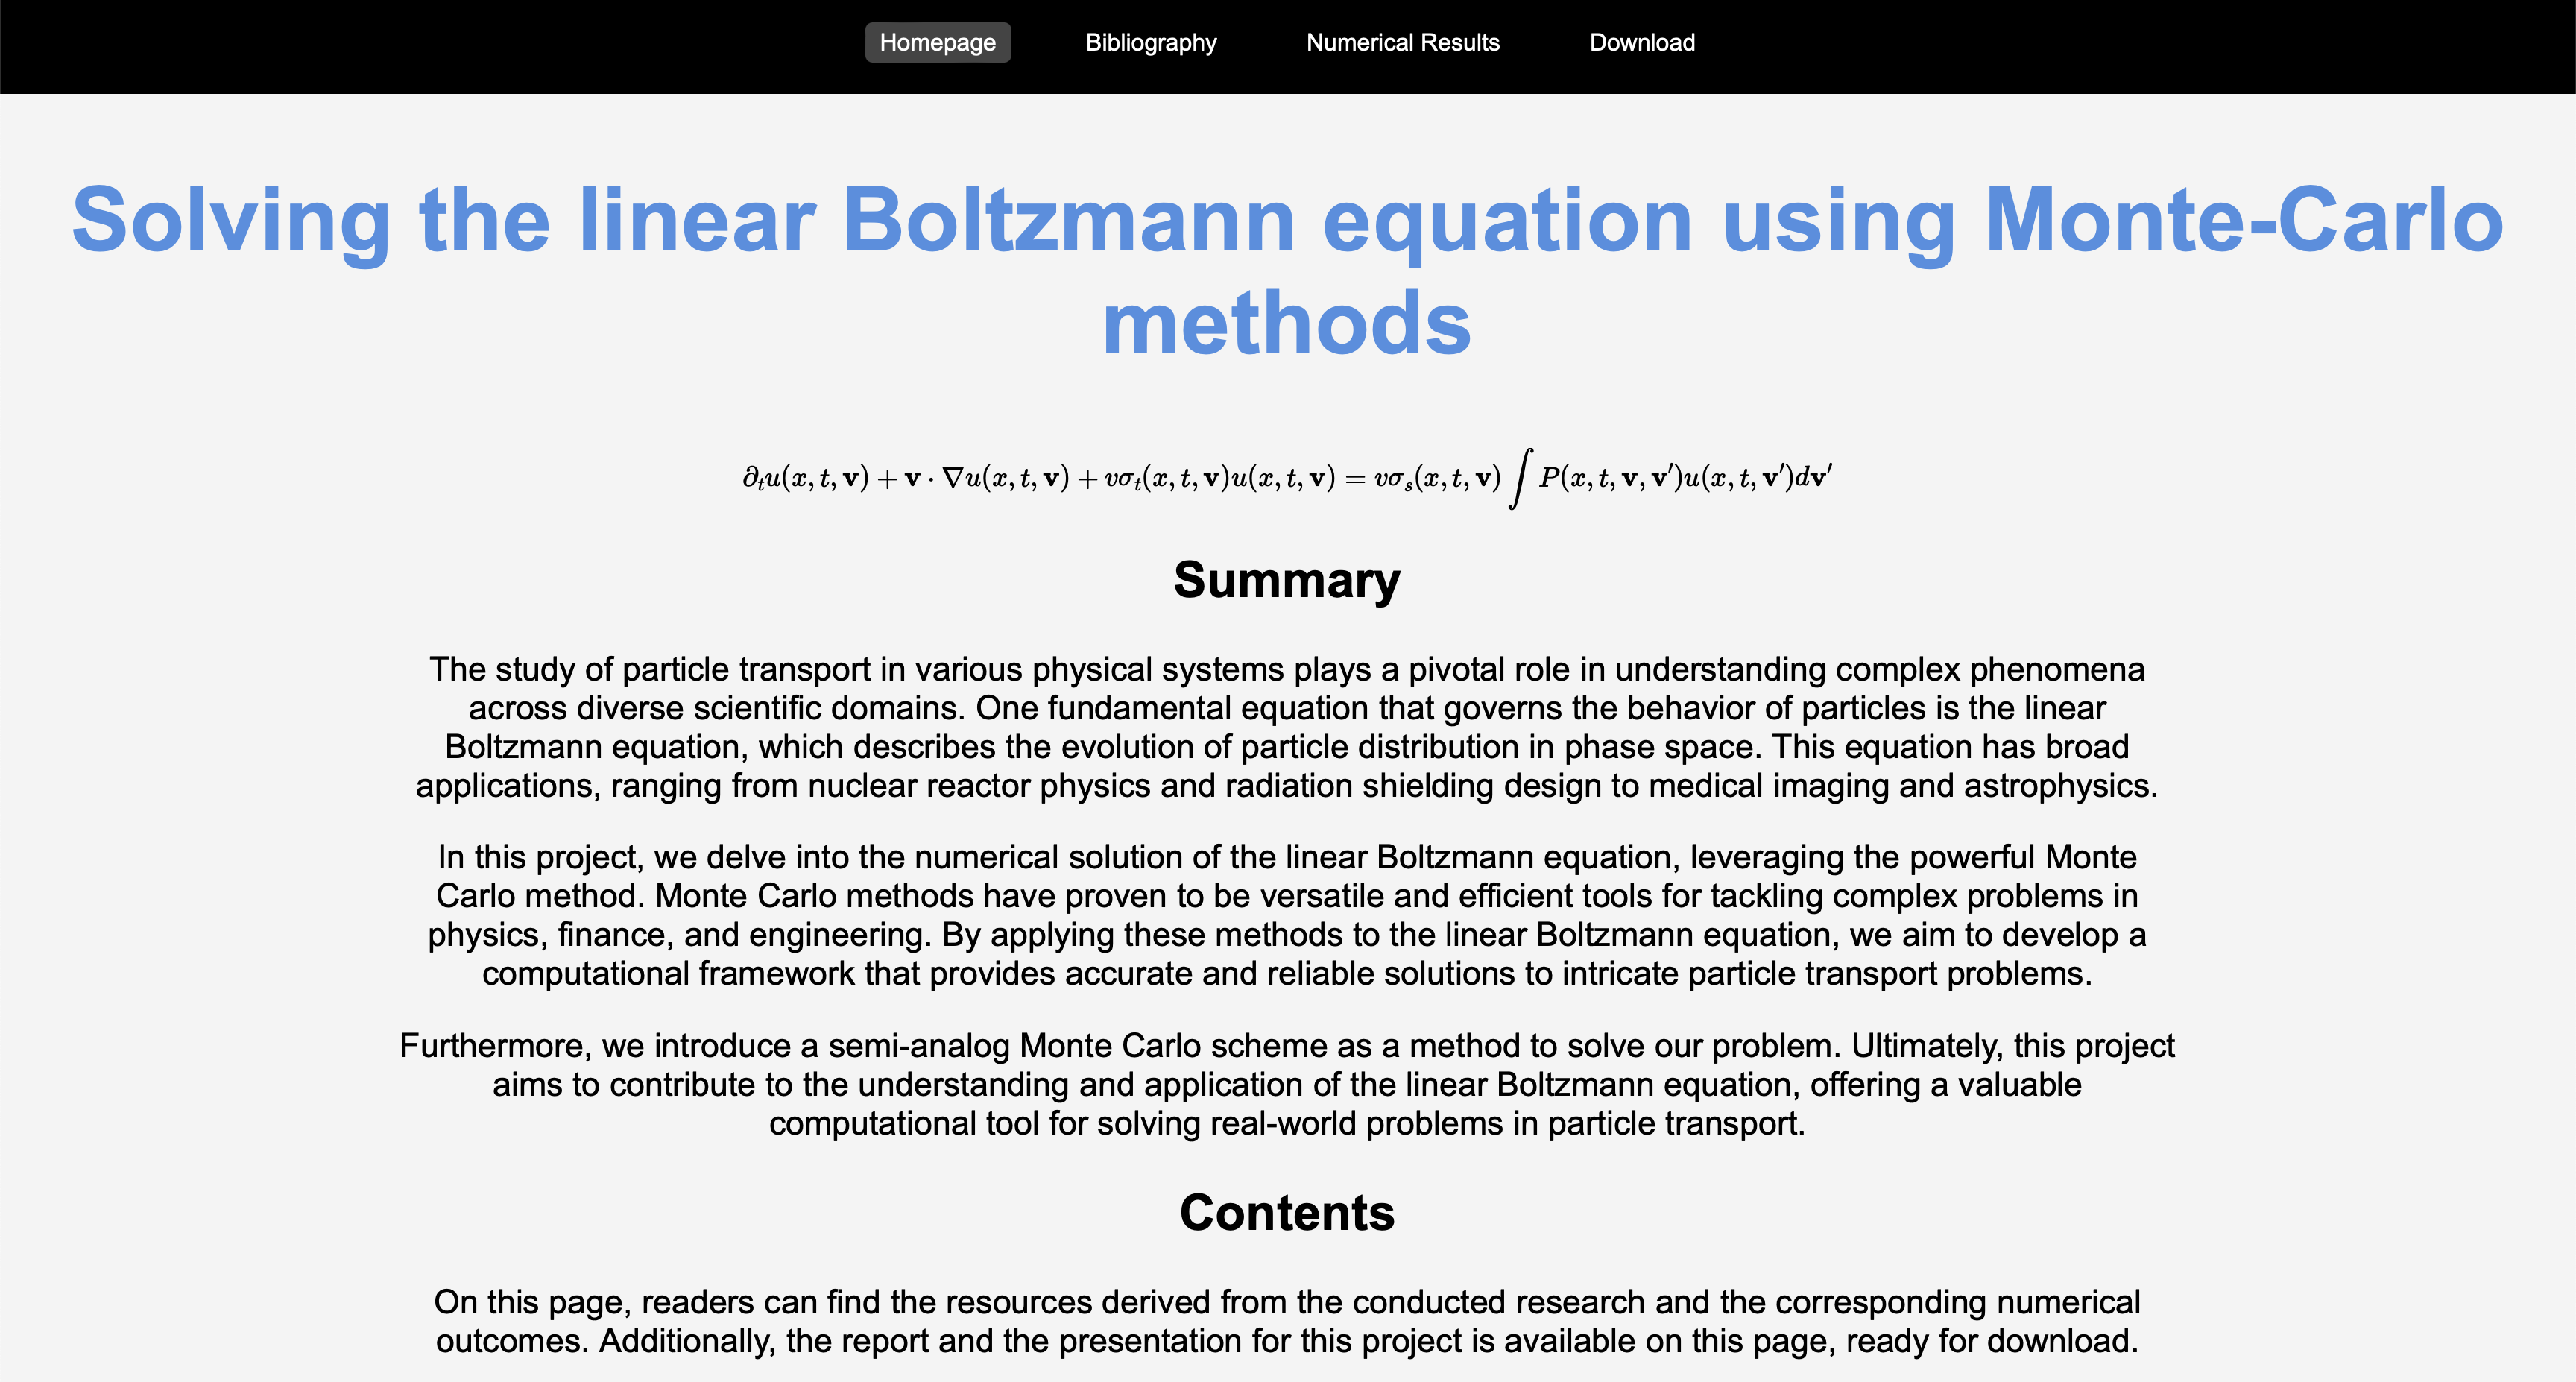
\includegraphics[height=0.7\textheight]{img/website.png}
	\end{figure}
	
	For further resources, only one adress:
	\centering
	\fbox{\color{IBMblue}\bfseries\href{https://clement16a.github.io/Boltzmann-Monte-Carlo-website/index.html}{Resolution of the linear Boltzmann equation by Monte Carlo method}}
\end{frame}

\begin{frame}[plain]{References}
	\setlength\bibitemsep{1.5\itemsep}
    \printbibliography
\end{frame}


\end{document}
